\documentclass[11pt]{article}
\usepackage[top=8mm, bottom=8mm, inner=8mm, outer=8mm, 
headheight=0mm, headsep=0mm, footskip=0mm, 
%papersize={148mm, 210mm},
papersize={297mm, 210mm},
includeheadfoot
]{geometry}
\usepackage{amsmath}
\usepackage{tikz}
\usepackage{lipsum}
\usepackage{fontspec}
\usepackage{xcolor}

\definecolor{past1}{HTML}{eaa6a5}
\definecolor{past2}{HTML}{ece1a5}
\definecolor{past3}{HTML}{bdeda5}
\definecolor{past4}{HTML}{a6edc9}
\definecolor{past5}{HTML}{a7b8ee}
\definecolor{past6}{HTML}{d0a6ee}

\definecolor{bold1}{HTML}{f52926}
\definecolor{bold2}{HTML}{f2d11c}
\definecolor{bold3}{HTML}{59ef0e}
\definecolor{bold4}{HTML}{1cf285}
\definecolor{bold5}{HTML}{184aeb}
\definecolor{bold6}{HTML}{9920ef}

\newcommand{\icon}[1]{{\setmainfont[Scale=1.3]{Chalkdust Icon Font}#1}\hspace{2pt}}

\def\UrlFont{\bfseries}
\newcommand{\linkfont}{}

\newcommand{\iconlink}[3][0mm]{\mbox{\hspace{#1}\icon{#2}\hspace{-#1}{\linkfont#3}}}
\newcommand{\unboxediconlink}[3][0mm]{\hspace{#1}\icon{#2}\hspace{-#1}{\linkfont#3}}

\newcommand{\twitter}[2][0mm]{\iconlink[#1]{a}{@#2}}
\newcommand{\facebook}[2][0mm]{\iconlink[#1]{b}{#2}}
\newcommand{\instagram}[2][0mm]{\iconlink[#1]{l}{#2}}
\newcommand{\myspace}[2][0mm]{\iconlink[#1]{f}{#2}}
\newcommand{\website}[2][0mm]{\iconlink[#1]{d}{#2}}
\newcommand{\youtube}[2][0mm]{\iconlink[#1]{m}{#2}}
\newcommand{\email}[2][0mm]{\iconlink[#1]{c}{#2}}
\newcommand{\postmail}[2][0mm]{\unboxediconlink[#1]{e}{#2}}
\newcommand{\mathstodon}[2][0mm]{\iconlink[#1]{n}{@#2@mathstodon.xyz}}
\newcommand{\stackexchange}[2][0mm]{\iconlink[#1]{o}{#2}}

\pagestyle{empty}

\setmainfont{Libertinus Sans}

\newcommand{\CDtitle}[1]{
{\setmainfont{Raleway SemiBold}\LARGE #1}\par
}

\setlength{\parskip}{6.8pt}

\newlength{\defaultparskip}
\setlength{\defaultparskip}{\parskip}

\setlength{\parindent}{0cm}

\newcommand{\CDsubtitle}[1]{
\par\medskip
{\setmainfont{Raleway SemiBold}\large #1}
\par
}

\begin{document}
\begin{minipage}[t][192mm]{132mm}
\CDtitle{How to pilot a punt}
\CDsubtitle{10 Get in the boat}
\vspace{-4mm}
\begin{center}
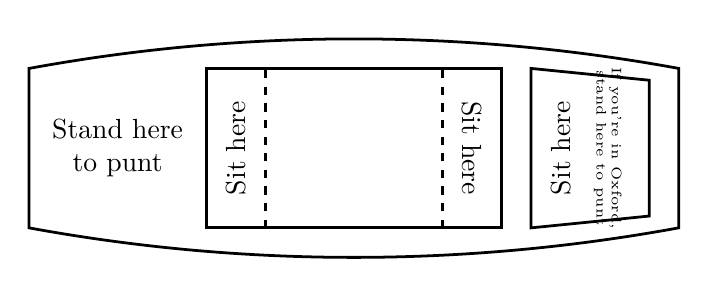
\begin{tikzpicture}[x=0.75cm,y=0.75cm]
%\draw[line width=1pt] (5,0) -- (5,2);
%\draw[line width=1pt] (0,0) -- (0,2);
\draw[line width=1pt] (0,0) arc (-100.39:-79.61:30.5) -- (11,0) -- (11,2.7) arc (79.61:100.39:30.5) -- (0,2.7) -- cycle;
\draw[line width=1pt] (3,0) rectangle (8,2.7);
\draw[line width=1pt] (8.5,0) -- (10.5,0.2) -- (10.5,2.5) -- (8.5,2.7) -- cycle;
\draw[line width=1pt,dashed] (7,0) -- (7,2.7);
\draw[line width=1pt,dashed] (4,0) -- (4,2.7);
\node[rotate=90] at (3.5,1.35) {Sit here};
\node[rotate=-90] at (7.5,1.35) {Sit here};
\node[rotate=90] at (9,1.35) {Sit here};
\node[align=center] at (1.5,1.35) {Stand here\\to punt};
\node[align=center,rotate=-90] at (9.8,1.35) {\tiny If you're in Oxford,\\[-2.3mm]\tiny stand here to punt};
%\draw[line width=2pt] (0,0) -- plot[domain=4.44:4.98,variable=\t]({2.5+1*9.34*cos(\t r)},{9 + 9.34*sin(\t r)});
\end{tikzpicture}
\end{center}

\vfill

\CDsubtitle{20 Drop the pole vertically into the water beside the boat}
\vspace{-3mm}
\begin{center}
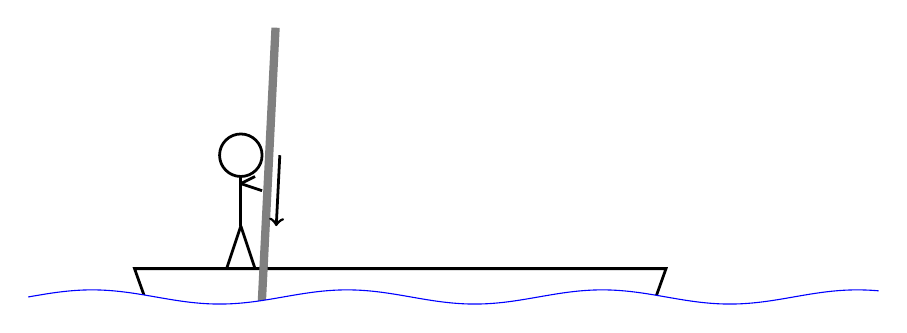
\begin{tikzpicture}[x=0.9cm,y=0.9cm]
\begin{scope}
\clip (0,3.8) -- plot[domain=0:12,samples=500,variable=\x] ({\x},{0.1*sin(\x*100)}) -- (12,3.8) -- cycle;
\draw[line width=1pt] (2,-1) -- (1.5,0.4) -- (9,0.4) -- (8.5,-1);
\draw[line width=1pt] (3,2) circle (0.3);
\draw[line width=1pt] (3,1.7) -- (3,1);
\draw[line width=1pt] (2.8,0.4) -- (3,1);
\draw[line width=1pt] (3.2,0.4) -- (3,1);
\draw[line width=1pt] (3,1.6) -- (3.2,1.7);
\draw[line width=3pt, gray] (3.49,3.8) -- (3.25,-1);
\draw[line width=1pt] (3.3,1.5) -- (3,1.6);
\end{scope}
\draw[blue] plot[domain=0:12,samples=500,variable=\x] ({\x},{0.1*sin(\x*100)});
\draw[line width=1pt,->] (3.55,2) -- (3.5,1);
\end{tikzpicture}
\end{center}

\vfill

\CDsubtitle{30 Catch pole and push forward off the bottom of the river}
\vspace{-6mm}
\begin{center}
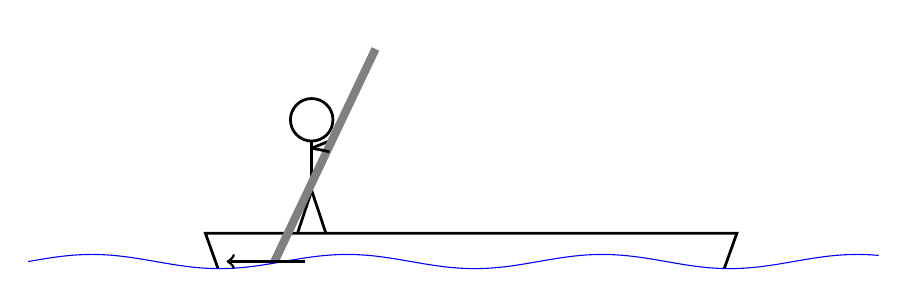
\begin{tikzpicture}[x=0.9cm,y=0.9cm]
\begin{scope}
\clip (0,3.3) -- plot[domain=0:12,samples=500,variable=\x] ({\x},{0.1*sin(\x*100)}) -- (12,3.3) -- cycle;
\begin{scope}[shift={(1,0)}]
\draw[line width=1pt] (2,-1) -- (1.5,0.4) -- (9,0.4) -- (8.5,-1);
\draw[line width=1pt] (3,2) circle (0.3);
\draw[line width=1pt] (3,1.7) -- (3,1);
\draw[line width=1pt] (2.8,0.4) -- (3,1);
\draw[line width=1pt] (3.2,0.4) -- (3,1);
\draw[line width=1pt] (3,1.6) -- (3.25,1.7);
\draw[line width=3pt, gray] (3.9,3) -- (2,-1);
\draw[line width=1pt] (3.25,1.55) -- (3,1.6);
\end{scope}
\end{scope}
\draw[blue] plot[domain=0:12,samples=500,variable=\x] ({\x},{0.1*sin(\x*100)});
\draw[line width=1pt,->] (3.9,0) -- (2.8,0);
\end{tikzpicture}
\end{center}

\vfill

\CDsubtitle{40 Let the boat glide along the river, using the pole to steer}
\begin{center}
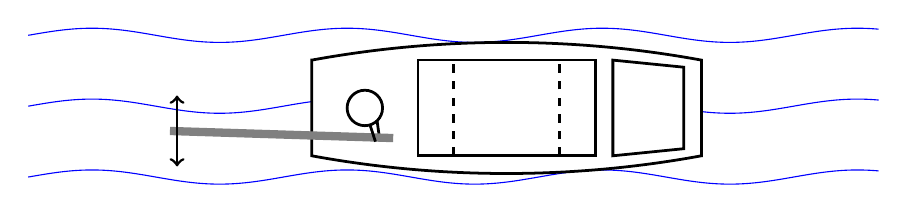
\begin{tikzpicture}[x=0.9cm,y=0.9cm]
\draw[blue] plot[domain=0:12,samples=500,variable=\x] ({\x},{0.1*sin(\x*100)});
\draw[blue] plot[domain=0:12,samples=500,variable=\x] ({\x},{1+0.1*sin(\x*100)});
\draw[blue] plot[domain=0:12,samples=500,variable=\x] ({\x},{2+0.1*sin(\x*100)});
\begin{scope}[shift={(4,0.3)},scale=0.5]
\draw[line width=1pt,fill=white] (0,0) arc (-100.39:-79.61:30.5) -- (11,0) -- (11,2.7) arc (79.61:100.39:30.5) -- (0,2.7) -- cycle;
\draw[line width=1pt] (3,0) rectangle (8,2.7);
\draw[line width=1pt] (8.5,0) -- (10.5,0.2) -- (10.5,2.5) -- (8.5,2.7) -- cycle;
\draw[line width=1pt,dashed] (7,0) -- (7,2.7);
\draw[line width=1pt,dashed] (4,0) -- (4,2.7);

\draw[line width=1pt] (1.8,1.31) -- (1.9,0.6);
\draw[line width=3pt, gray] (2.3,0.5) -- (-4,0.7);
\draw[line width=1pt] (1.5,1.31) -- (1.8,0.4);
\draw[line width=1pt,fill=white] (1.5,1.35) circle (0.5);
\draw[line width=1pt,<->] (-3.8,-0.3) -- (-3.8,1.7);
\end{scope}
\end{tikzpicture}
\end{center}

\vfill

\CDsubtitle{50 Lift pole upwards out of water}

\vfill

\CDsubtitle{60 GOTO 20}

\end{minipage}%
\hfill%
\begin{minipage}[t][192mm]{132mm}
\setlength{\parskip}{\defaultparskip}

\CDtitle{TMiP 2019 treasure punt}
Four mathematicians---Ben, Katie, Kevin, and Sam---each have one of the four clues needed to unlock a great treasure.
On a sunny/cloudy/rainy/snowy (delete as appropriate) they met up in Cambridge to go punting, share their clues, work out the combination for the lock,
and share out the treasure. One or more of the mathematicians, however, had decided to lie about their clue so they could steal all the treasure for themselves.
At least one mathematician is telling the truth.*


They met at Cambridge Chauffeur Punts, and headed North under Silver Street Bridge. Ben pointed out a plaque on the bridge with two years written on it:

``My clue,'' he said, ''told me that the sum of the digits of the code is equal to the sum of the digits of the earlier year on that plaque. My clue also told me that one of the digits of the code is 7.''
%1702

The mathematicians next punted under the mathematical bridge, gasping in awe at its tangential trusses, then punted along the river under King's College Bridge and past King's College.
Katie pointed to a sign on the King's College lawn near the river:

``See that sign whose initials are PNM?'' said Katie. ``My clue stated that first digit of the code is equal to the number of vowels on that sign.
My clue also told me that one of the digits of the code is 1.''
%7

They then reached Clare Bridge. Kevin pointed out the spheres on Clare bridge:

``My clue'' he said, ``stated that the number of spheres on (both sides of) this bridge is a factor of the code. My clue also told me that one of the digits of the code is 3.''
%14
(Kevin had not noticed that one of the spheres had a wedge missing, so had counted that as a whole sphere.)

They continued to punt past Clare College. Just before they reached Garret Hostel Bridge, Sam pointed out the Jerwood Library and a sign showing the year it was built:

``My clue'' she said, ``said that the largest prime factor of that year appears$^\text{†}$ in the code.
My clue also said that the smallest prime factor of that year appears in the code. My clue also told me that one of the digits of the code is 2.''
%1998''

They then punted under Garret Hostel Bridge, turned around between it and Trinity College Bridge, and headed back towards Cambridge Chauffeur Punts.
The lies confused them and they couldn't unlock the treasure. Can you work out who was lying and claim the treasure for yourself?

\vfill

{\footnotesize *If the mathematicians say multiple sentences about their clue, then they are either all true or all false.\\[-1mm]
$^\text{†}$In the same was as you might say the number 18 appears in 1018 or 2189.}
\end{minipage}

\newpage

\CDtitle{TMiP 2019 treasure punt map}
\begin{tikzpicture}
%\node[anchor=south west] at (0,0) {\includegraphics[width=28cm]{map.png}};

\path (0,2.2) arc (270:310:8) arc (130:90:10) coordinate(C) -- (28,6.6);
\path (0,5.2) arc (210:310:2.4) arc (130:90:15) coordinate(B) -- (28,8.2);

\begin{scope}
\clip (0,5.2) arc (210:310:2.4) arc (130:90:15) -- (28,8.2) -- (28,6.6) -- (C) arc (90:130:10) arc (310:270:8) -- cycle;
%\foreach \x in {0,...,50}
%    \draw[blue] plot[domain=0:9,samples=500,variable=\y] ({0.5*\x+0.3+0.1*sin(\y*400)},{\y});
\end{scope}

\begin{scope}
\clip (0,9.2) arc (210:310:2.4) arc (130:90:15) -- (28,12.2) -- (28,8.2) -- (B) arc(90:130:15) arc (310:210:2.4) -- cycle;
\fill[color=past1] (3.5,3.8) -- (-4,20) -- (3,20) -- (17,0) -- cycle;
\node[rotate=26,white] at (6.3,8.2) {\setmainfont{Raleway SemiBold}\Large Queen's College};
\fill[color=past5] (12,0) -- (12,20) -- (18.5,20) -- (18.5,0) -- cycle;
\node[white] at (15.4,10.2) {\setmainfont{Raleway SemiBold}\Large King's College};
\fill[color=past4] (23,0) -- (23,20) -- (18.7,20) -- (18.7,0) -- cycle;
\node[white] at (20.85,10.2) {\setmainfont{Raleway SemiBold}\Large Clare College};
\fill[color=past6] (23.3,0) -- (23.3,20) -- (28,20) -- (28,0) -- cycle;
\node[white] at (25.65,10.2) {\setmainfont{Raleway SemiBold}\Large Trinity Hall};
\end{scope}

\begin{scope}
\clip (0,-1.8) arc (270:310:8) arc (130:90:10) -- (28,2.6) -- (28,6.6) -- (C) arc (90:130:10) arc (310:270:8) -- cycle;
\fill[color=past1] (3.5,3.8) -- (12,-5) -- (14,-10) -- (10,20) -- cycle;
\fill[color=past5] (18.5,8) -- (18.5,-5) -- (14.3,-10) -- (10.3,20) -- cycle;
\fill[color=past4] (18.7,8) -- (18.7,-5) -- (21,-10) -- (21,20) -- cycle;
\fill[color=past6] (21,8) -- (21,-5) -- (28,-10) -- (28,20) -- cycle;
\end{scope}

\draw[gray,line width=2pt] (0,5.2) arc (210:310:2.4) arc (130:90:15) -- (28,8.2);
\draw[gray,line width=2pt] (0,2.2) arc (270:310:8) arc (130:90:10) -- (28,6.6);

\fill[white] (2,4.5) -- (3.8,2.5) -- (4.1,2.8) -- (2.3,4.8) -- cycle;
\draw[line width=1pt] (2,4.5) -- (3.8,2.5);
\draw[line width=1pt] (2.3,4.8) -- (4.1,2.8);
\node[rotate=-48] at (3.05,3.65) {\small Silver Street Bridge};

\fill[past1] (4,5.5) -- (5.3,3.5) -- (5.6,3.725) -- (4.3,5.725) -- cycle;
\draw[line width=1pt] (4,5.5) -- (5.3,3.5);
\draw[line width=1pt] (4.3,5.725) -- (5.6,3.725);
\node[rotate=-57] at (4.8,4.6125) {\small Mathematical Bridge};

\fill[past5] (12.3,8.5) -- (12.3,6) -- (12.7,6) -- (12.7,8.5) -- cycle;
\draw[line width=1pt] (12.3,8.5) -- (12.3,6);
\draw[line width=1pt] (12.7,8.5) -- (12.7,6);
\node[rotate=-90] at (12.5,7.25) {\small King's College Bridge};

\fill[past4] (18.8,8.5) -- (18.8,6) -- (19.2,6) -- (19.2,8.5) -- cycle;
\draw[line width=1pt] (18.8,8.5) -- (18.8,6);
\draw[line width=1pt] (19.2,8.5) -- (19.2,6);
\node[rotate=-90] at (19,7.25) {\small Clare Bridge};

\fill[white] (23,8.4) -- (24.4,6.1) -- (25.1,4.65) -- (25.1,0) -- (25.5,0) -- (25.5,4.8) -- (24.7,6.3) -- (23.3,8.6) -- cycle;
\draw[line width=1pt] (23,8.4) -- (24.4,6.1);
\draw[line width=1pt] (23.3,8.6) -- (24.7,6.3);
\node[rotate=-58.5] at (23.85,7.35) {\small Garret Hostel Bridge};

\fill[past6] (27.9,8.7) -- (27.9,6.2) -- (27.5,6.2) -- (27.5,8.7) -- cycle;
\draw[line width=1pt] (27.5,8.7) -- (27.5,6.2);
\draw[line width=1pt] (27.9,8.7) -- (27.9,6.2);
\node[rotate=-90] at (27.7,7.45) {\small Trinity College Bridge};

\begin{scope}[shift={(26.7,2)}]
\draw[line width=1pt,->] (-0.4,0) -- (0.6,0) node[anchor=west] {N};
\draw[line width=1pt] (0,-0.4) -- (0,0.4);
\fill (0,0) circle (0.1);
\end{scope}

\newcommand{\nodetext}[3][5cm]{
\begin{minipage}{#1}\null\hfill\textbf{#2}\hfill\null\\#3\end{minipage}
}
\newcommand{\nodetextnotitle}[2][5cm]{
\begin{minipage}{#1}#2\end{minipage}
}

\draw[->,line width=2pt] (3,10) node[anchor=south,align=center,inner sep=1pt] {\nodetext[4.5cm]{START}{Pick up your punt from Cambridge Chauffeur Punts}} -- (1.8,4.5);
\draw[->,line width=2pt] (6,3) node[anchor=west,align=center,inner sep=1pt] {Ben's clue} -- (3.5,3.8);
\draw[->,line width=2pt] (16,5) node[anchor=north,align=center,inner sep=1pt] {Katie's clue} -- (15.75,6.3);
\draw[->,line width=2pt] (17.8,9) node[anchor=south,align=center,inner sep=1pt] {Kevin's clue} -- (18.7,7.75);
\draw[->,line width=2pt] (23.5,5.5) node[anchor=north east,align=center,inner sep=1pt] {Sam's clue} -- (24.1,6.4);

%\path (0,2.2) arc (270:310:8) arc (130:90:10) coordinate(C) -- (28,6.6);
%\path (0,5.2) arc (210:310:2.4) arc (130:90:15) coordinate(B) -- (28,8.2);
\draw[->,line width=2pt] (25.8,7.8) -- (26,7.8) arc (90:-90:0.4) -- (25.8,7);
\node[anchor=north west] at (0,1) {\CDsubtitle{\color{gray}Space for taking notes/working out}};
\node[anchor=south east] at (28,-6.3) {\begin{minipage}{10cm}
\begin{center}\includegraphics[width=10cm]{chalkdust-logo-black-on-white.jpg}\end{center}

\vspace{-8mm}

This treasure punt was written by the team behind Chalkdust, a magazine for the mathematically curious.
Find out more by reading the copy of Chalkdust that you were given in your TMiP welcome pack.
Talk to us after punting about how to write for Chalkdust.

\begin{center}
\website{chalkdustmagazine.com}
\quad
\twitter{chalkdustmag}
\quad
\facebook{chalkdustmag}
\quad
\instagram{chalkdustmag}
\quad
\myspace{chalkdustmag}
\end{center}
\end{minipage}};
\end{tikzpicture}


\end{document}
